\documentclass[11pt]{article}
\usepackage[utf8]{inputenc}	% Para caracteres en español
\usepackage{amsmath,amsthm,amsfonts,amssymb,amscd}
\usepackage{multirow,booktabs}
\usepackage[table]{xcolor}
\usepackage{fullpage}
\usepackage{lastpage}
\usepackage{enumitem}
\usepackage{fancyhdr}
\usepackage{mathrsfs}
\usepackage{wrapfig}
\usepackage{setspace}
\usepackage{hyperref}
\usepackage{calc}
\usepackage{multicol}
\usepackage{cancel}
\usepackage[retainorgcmds]{IEEEtrantools}
\usepackage[margin=3cm]{geometry}
\usepackage{amsmath}
\newlength{\tabcont}
\setlength{\parindent}{0.0in}
\setlength{\parskip}{0.05in}
\usepackage{empheq}
\usepackage{framed}
\usepackage[most]{tcolorbox}
\usepackage{xcolor}
\colorlet{shadecolor}{orange!15}
\parindent 0in
\parskip 12pt
\geometry{margin=1in, headsep=0.25in}
\theoremstyle{definition}
\usepackage{pdfpages}
\newtheorem{defn}{Definition}
\newtheorem{reg}{Rule}
\newtheorem{exer}{Exercise}
\newtheorem{note}{Note}
\usepackage{fancyhdr}\usepackage{xcolor}\usepackage{amsmath}\usepackage{amssymb}\pagestyle{fancy}\rhead{}
\newtheorem{theorem}{Theorem}[subsection]
\theoremstyle{definition}
\newtheorem{definition}[theorem]{Definiton}
\newtheorem{example}[theorem]{Example}
\newtheorem{corollary}[theorem]{Corollary}
\newtheorem{lemma}[theorem]{Lemma}
\title{Chapter 9 Review Notes}

\begin{document}
\thispagestyle{empty}
{\LARGE \bf ECE 159 Lecture Notes}\\
{\large Hei Shing Cheung}\\
Fundamentals of Electric Circuits, Winter 2024 \hfill ECE 159\\
\\
The up-to-date version of this document can be found at \url{https://github.com/HaysonC/skulenotes}\\
\vspace{10pt}
\section{Basic Concepts}
\paragraph{} One should have understood, after the course of high school physics, the basic concepts of electric circuits. This includes the concepts of voltage, current, resistance, and power. In this course, we will be building upon these concepts and applying them to more complex circuits. 
\subsection{Basic Defintions}
\begin{definition}[Voltage]
    The difference of the electric potential between two points in a circuit. The enegy required to move a charge from one point to another.
    \begin{equation}
        V \defeq \int_C \textbf{E} \cdot d\textbf{l} = \frac{dW}{dq}
    \end{equation}
    \end{definition}
    \paragraph{Polarity} The polarity is fliped as illustrated when the voltage is indicated as negative.
    \begin{definition}[Current]
    Rate of change of charge at a particular point in the circuit.
    \begin{equation}
        I \defeq \frac{dq}{dt}
    \end{equation}
    \end{definition}
    
    \begin{definition}[Power]
    The rate of change of energy for an element in the circuit. Power is the product of voltage and current.
    \begin{equation}
        P \defeq \frac{dW}{dt} = \frac{dW}{dq} \cdot \frac{dq}{dt} = V \cdot I
    \end{equation}
    \end{definition}
    
    \begin{definition}[Resistors]
    A circuit element that restricts the flow of charge.
    \end{definition}
    
    \begin{definition}[Ideal Sources]
    A circuit element that provides a set voltage or current regardless of what it is connected to.
    \end{definition}
    
    \begin{definition}[Dependent Sources]
    A circuit element that provides a voltage or current to the circuit depending on another voltage or current in the circuit.
    \end{definition}
    
    \begin{definition}[Passive Sign Convention]
    If a positive current flows out of the positive side of a voltage, that element is \textbf{delivering} power. Otherwise, it is \textbf{absorbing} power. All resistors absorb power.
    \end{definition}
\subsection{High School Review}
\paragraph{Electric Field} $\textbf{E}$ is created when charges are separated. It leads to a potential difference.
\paragraph{Worked done by Electric Field} Force due to the field is:
\begin{equation}
    \textbf{F} = q\textbf{E}
\end{equation}
, such that it moves charges and do work.
\paragraph{Capacitor} Energy stored in capacity is:
\begin{equation}
    U_\text{E} = \frac{1}{2}CV^2
\end{equation}
\paragraph{Energy Density} The energy [J/m$^3$] in a dielectric material is:
\begin{equation}
    u_\text{E} = \frac{1}{2}\epsilon_r \epsilon_0 E^2
\end{equation}
where:
\begin{center}
    $\epsilon_0$ = Permittivity of free space \\
    $\epsilon_r$ = Relative Permittivity
\end{center}
\paragraph{Magnetic field} \textbf{B} is created when charges move.
\paragraph{An electromotive force (emf)} can be induced when the magnetic flux
through a loop is changing with time. Induced emf does the same thing as the potential difference of a
battery. 
\paragraph{Induced EMF} An inductor can store energy in a ``magnetic form"
\begin{equation}
    U_B = \frac{1}{2} L i^2 \quad 
\end{equation}
\paragraph{Energy Density}
\begin{equation}
    u_B = \frac{1}{2 \mu_r \mu_0} B^2
\end{equation}
\subsection{Voltage and Current}
\paragraph{} Now instead of dealing with electric and magnetic vector fields, we can
use the scalar quantities of voltage and current:
\begin{align}
    \text{Voltage} &\defeq \text{Difference in Electric Potential}\nonumber \\ 
    \Delta V &= V_A - V_B \nonumber \\
    &= \int_B^A \textbf{E} \cdot dl \nonumber\\
    &= \frac{\Delta W}{q}
\end{align}

\paragraph{Electromotive Force (emf) / Voltage} Work is performed by 
the electric field to move a charge from one point to another. 
The work done per unit charge is the voltage.
\begin{equation}
    \text{Voltage} = \frac{\Delta W}{q}
\end{equation}
\subsection{Power and Energy}
\paragraph{Power} To relate power to  voltage and current, we can use the following equation:
\begin{equation}
    P \defeq \frac{dW}{dt} = \frac{dW}{dq} \cdot \frac{dq}{dt} = V \cdot I
\end{equation}
\paragraph{Sign} If $P = V \cdot I > 0$, the element is delivering power. If $P = V \cdot I < 0$, the element is absorbing power.
\paragraph{Energy}  the energy absorbed or supplied by an element
from time $t_0$ to time $t_1$ is:
\begin{equation}
    W = \int_{t_0}^{t_1} P(t) dt
\end{equation}
\paragraph{} The above concepts might be revisited in the future, but it is important to understand the basic concepts of voltage, current, resistance, power, and energy.
\section{Basic DC Circuit Analysis with Resistors and Sources}
\subsection{Circuit Elements}
\paragraph{Active Elements} Active elements are sources of energy. They can deliver power to the circuit. While passive elements are elements that can only absorb power.
\paragraph{Ideal Sources} Ideal sources are sources that provide a set voltage or current regardless of what it is connected to. We often assume that sources are ideal.
\paragraph{Independent Sources} Independent sources are sources that provide a set voltage or current regardless of what it is connected to.
\paragraph{Dependent Sources} Dependent sources are sources that provide a voltage or current to the circuit depending on another voltage or current in the circuit.
\paragraph{Resistor} A resistor is a circuit element that restricts the flow of charge. The voltage across a resistor is proportional to the current through it.
\paragraph{Passive Sign Convention} If a positive current flows out of the positive side of a voltage, that element is delivering power. Otherwise, it is absorbing power. All resistors absorb power.
\subsection{Resistance}
\paragraph{Ohm's Law} Ohm's Law states that the current through a resistor is proportional to the voltage across it.
\begin{equation}
    V = IR
\end{equation}
\paragraph{Resistivity} The resistance of a material is proportional to the length of the material and inversely proportional to the cross-sectional area of the material.
\begin{equation}
    R = \rho \frac{l}{A}
\end{equation}
\paragraph{Short and Open Circuits} A short circuit is a circuit with no resistance, while an open circuit is a circuit with infinite resistance.
\paragraph{Conductance} The reciprocal of resistance is conductance. The unit of conductance is mho (ohm spelled backwards), \rotatebox[origin=c]{180}{$\Omega$}.
\begin{equation}
    G = \frac{1}{R}
\end{equation}
\paragraph{Power in Resistors} The power dissipated in a resistor is given by:
\begin{equation}
    P = I^2R = \frac{V^2}{R}
\end{equation}
\paragraph{Resistors in Series} If resistors are placed in series with each other, their current must be the same, The equivalent resistance of resistors in series is the sum of the resistances.
\begin{equation}
    R_{\text{eq}} = R_1 + R_2 + \dots + R_n
\end{equation}
\paragraph{Resistors in Parallel} If resistors are placed in parallel with each other, their voltage must be the same. The equivalent resistance of resistors in parallel is the reciprocal of the sum of the reciprocals of the resistances.
\begin{equation}
    \frac{1}{R_{\text{eq}}} = \frac{1}{R_1} + \frac{1}{R_2} + \dots + \frac{1}{R_n}
\end{equation}
\paragraph{Comination of Series and Parallel Resistors} To find the equivalent resistance of a combination of series and parallel resistors, first find the equivalent resistance of the resistors in series, then find the equivalent resistance of the resistors in parallel.
\paragraph{Voltage Division} The voltage across a resistor in series is proportional to the resistance of the resistor.
\begin{equation}
    V_i = V \frac{R_i}{R_{\text{eq}}}
\end{equation}
\paragraph{Current Division} The current through a resistor in parallel is proportional to the conductance of the resistor.
\begin{equation}
    I_i = I \frac{G_i}{G_{\text{eq}}} = I \frac{1}{R_i} \frac{1}{\sum \frac{1}{R_i}}
\end{equation}
\subsection{Node, Branch, and Loop}
\paragraph{} Three important ideas in electric circuit analysis are:
\begin{enumerate}
    \item \textbf{Branch}: A branch is an element in an electric circuit, such as a source or a resistor.
    \item \textbf{Node}: A point of connection of two or more branches within an electric circuit.
    \item \textbf{Loop}: Any closed path in an electric circuit. To form a loop, one must start and end at the same point and never pass through the same node twice.
\end{enumerate}
\subsection{Kirchhoff's Laws}
\paragraph{} Kirchhoff's Laws are two laws that are used to analyze electric circuits.
\paragraph{Kirchhoff's Current Law (KCL)} The sum of currents entering a node is equal to the sum of currents leaving a node.
\begin{equation}
    \sum I_{\text{in}} = \sum I_{\text{out}} \quad \text{or} \quad \sum_\text{$n$ in node} I_n = 0
\end{equation}
\paragraph{Kirchhoff's Voltage Law (KVL)} The sum of voltages around a closed loop is equal to zero.
\begin{equation}
    \sum_\text{$n$ in loop} V_{n} = 0
\end{equation}
\subsection{Nodal Analysis}
\paragraph{Nodal Analysis} Nodal analysis is a method used to analyze electric circuits. It involves writing Kirchhoff's Current Law for each node in the circuit.
\paragraph{Steps for Nodal Analysis}
\begin{enumerate}
    \item Identify the nodes in the circuit.
    \item Assign a voltage to each node.
    \item Write Kirchhoff's Current Law for each node.
    \item Solve the resulting system of equations.
\end{enumerate}
\paragraph{Supernode} A supernode is a combination of two nodes in a circuit. It is used to simplify the analysis of the circuit. A supernode is identified by a voltage source between two nodes or two nodes are shorted together.
\begin{example}[Supernode]
Consider the following circuit, where $V_s$ is a voltage source across two nodes.
\end{example} 
\begin{center}
\begin{circuitikz}
    \draw (0,0) to[V, v=$V_s$] (0,2) to[R, l=$R_1$] (2,2) to[R, l=$R_2$] (2,0) to[short] (0,0);
\end{circuitikz}
\end{center} 
    \begin{align*}
        V_1 - V_2 &= V_s  \\
        \frac{V_1 - V_2}{R_1} + \frac{V_2}{R_2} &= 0
    \end{align*}
\paragraph{Strategies} When solving nodal analysis problems, it is important to choose a good ground node, most likely a question consist of two nodes equation with one or two addition simple equation.
\subsection{Mesh Analysis}
\paragraph{Mesh Analysis} Mesh analysis is a method used to analyze electric circuits. It involves writing Kirchhoff's Voltage Law for each loop in the circuit.
\paragraph{Steps for Mesh Analysis}
\begin{enumerate}
    \item Identify the loops in the circuit.
    \item Assign a current to each loop.
    \item Write Kirchhoff's Voltage Law for each loop.
    \item Solve the resulting system of equations.
\end{enumerate}
\paragraph{Supermesh} A supermesh is a combination of two loops in a circuit. It is used to simplify the analysis of the circuit. A supermesh is identified by a current source between two loops or two loops are shorted together.
\begin{example}[Supermesh]
Consider the following circuit, where $I_s$ is a current source between two loops.
\end{example}
\begin{center}
    \begin{circuitikz}
        \draw
        (0,0) to[R, l=$R_1$] (0,3) -- (2,3) to[R, l=$R_2$] (2,0) -- (0,0)
        (2,3) -- (4,3) to[R, l=$R_3$] (4,0) -- (2,0)
        (0,3) to[I, l=$I_s$] (4,3);
    \end{circuitikz}
\end{center}
\begin{align*}
    \text{Mesh 1:} & \quad -V_1 + I_1 R_1 + I_1 R_2 - I_s R_2 = 0 \\
    \text{Mesh 2:} & \quad -V_2 + I_2 R_3 + I_2 R_2 + I_s R_2 = 0 \\
    \text{Supermesh:} & \quad I_1 - I_2 = I_s
    \intertext{Addtionally, we can consider the entire circuit (or any loop that includes the current source) as a supermesh.}
\end{align*}
\paragraph{Strategies} When solving mesh analysis problems, it is important to choose a good loop, and to avoid current sources in the loop.
\subsection{Superpostion, Tricks and Equivalent Circuits}
\paragraph{Superposition} Superposition is a method used to analyze electric circuits. It involves analyzing the circuit with each source individually.
\paragraph{Steps for Superposition}
\begin{enumerate}
    \item Turn off all sources except one. (voltage sources are shorted, current sources are open)
    \item Analyze the circuit with the one source.
    \item Repeat for each source.
    \item Add the results together.
\end{enumerate}
\paragraph{Circuit of Dependent Sources} If a cicuit is composed of entirely dependent sources, the circuit has no current or voltage. However, we might be asked to find the equivalent resistance of the circuit, which can be done by applying a test voltage or current. 
\paragraph{Nodal Analysis by Inspection} We can create a matrix of conductances and voltages to solve for the nodal voltages. The diagonal elements are the sum of the conductances connected to the node, while the off-diagonal elements are the negative conductance between the nodes.
\begin{theorem}[Thevenin's Theorem]
    Thevenin's Theorem states that any linear circuit can be replaced by an equivalent circuit consisting of a voltage source and a resistor.
    \begin{equation}
        V_{\text{th}} = V_{\text{oc}} \quad R_{\text{th}} = R_{\text{eq}}
    \end{equation}
\end{theorem}
\begin{theorem}[Norton's Theorem]
    Norton's Theorem states that any linear circuit can be replaced by an equivalent circuit consisting of a current source and a resistor.
    \begin{equation}
        I_{\text{N}} = I_{\text{sc}} \quad R_{\text{N}} = R_{\text{eq}}
    \end{equation}
\end{theorem} 
\paragraph{Thevenin Resistance} The Thevenin resistance is the resistance seen by the load resistor when the load resistor is removed (V = 0 and I open). There are cases we could consider:
\begin{enumerate}
    \item If there is only independent sources, then we simply remove the sources and find the equivalent resistance.
    \item If there is only dependent sources, then we could apply a test voltage or current to find the equivalent resistance.
    \item If there is a combination of independent and dependent sources, we could apply a test voltage or current to find the equivalent resistance after removing the independent sources.
\end{enumerate}
The above theorems are direct results of each other.
\begin{example}[Thevenin's Theorem]
    Consider the following circuit, where we are asked to find the Thevenin equivalent circuit.
    \end{example}
    \begin{center}
\begin{circuitikz}
    \draw
    (0,0) to[V, v=$V_s$] (0,3) -- (2,3) to[R, l=$R_1$] (2,0) -- (0,0)
    (2,3) -- (4,3) to[R, l=$R_2$] (4,0) -- (2,0)
    (4,3) -- (6,3) to[R, l=$R_L$] (6,0) -- (4,0)
    (2,0) -- (2,-2) to[I, l=$I_s$] (4,-2) -- (4,0);
\end{circuitikz}
\end{center}
We remove the voltage and current sources and find the equivalent resistance.
\begin{center}
\begin{circuitikz}
    \draw
    (0,0) -- (0, 3) -- (2,3) to[R, l=$R_1$] (2,0) -- (0,0)
    (2,3) -- (4,3) to[R, l=$R_2$] (4,0) -- (2,0)
    (4,3) -- (6,3) to[R, l=$R_L$] (6,0) -- (4,0)
    (2,0) -- (2,-2) to[open, i^=$I_s$] (4,-2) -- (4,0);
\end{circuitikz}
\end{center}
\begin{theorem}[Maximum Power Transfer Theorem]
    The maximum power transfer theorem states that the maximum power is transferred to the load resistor when the load resistor is equal to the Thevenin resistance.
    \begin{equation}
        R_L = R_{\text{th}}
    \end{equation}
\end{theorem}
\section{Operational Amplifiers}
\begin{definition}[Operational Amplifier (Op-Amp)]
    An operational amplifier is a high-gain electronic voltage amplifier with a differential input and, usually, a single-ended output.
\end{definition}
\subsection{Ideal Op-Amp}
\paragraph{Ideal Op-Amp} An ideal op-amp has the following characteristics:
\begin{enumerate}
    \item $V_+ = V_-$
    \item $I_+ = I_- = 0$
\end{enumerate}
\paragraph{Common Op-Amp Circuits} There are several common op-amp circuits that are used in electric circuits. They could be found in the appendix \ref{app:opampcircuits}.
\section{First Order Circuits}
\begin{definition}[First Order Circuits]
    A first order circuit is a circuit that can be described by a first order differential equation.
\end{definition}
\appendix
\newpage
\rhead{CIV Formula Booklet}
\lhead{\leftmark}
\pagenumbering{alph}

\section{Common Op-Amp Circuits} \label{app:OpAmpCircuits}
\begin{figure}[h!]
    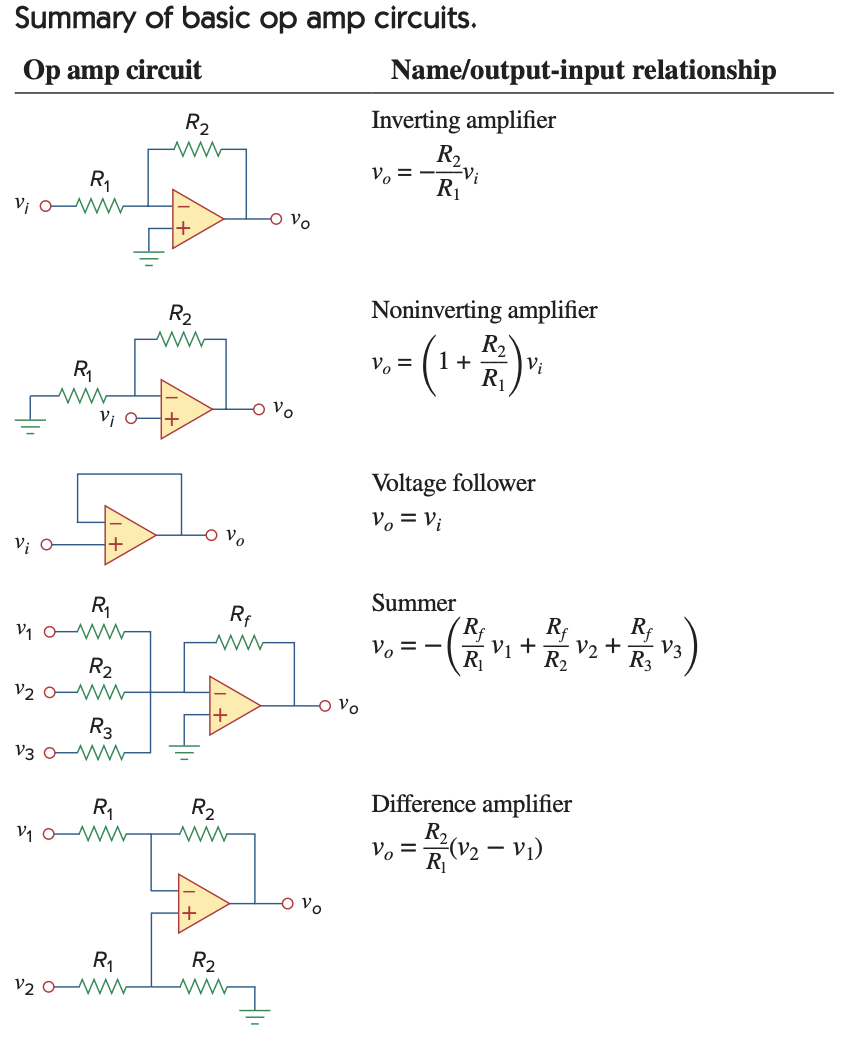
\includegraphics[width=0.9\linewidth]{AppendixItems/OpAmps.png}
    \centering
    \caption{Common Op-Amp Circuits}
\end{figure}
\end{document}